\documentclass{article}
\usepackage{listings}
\usepackage{mathrsfs}
\usepackage[utf8]{inputenc}
\usepackage{amssymb}
\usepackage{lipsum}
\usepackage{amsmath}
\usepackage{fancyhdr}
\usepackage{geometry}
\usepackage{scrextend}
\usepackage[english,german]{babel}
\usepackage{titling}
\setlength{\droptitle}{-3cm}
\usepackage{tikz}
\usepackage{algorithm,algpseudocode}
\usepackage[doublespacing]{setspace}
\usetikzlibrary{datavisualization}
\usetikzlibrary{datavisualization.formats.functions}
\usepackage{polynom}
\usepackage{amsmath}
\usepackage{gauss}
\usepackage{tkz-euclide}
\usetikzlibrary{datavisualization}
\usetikzlibrary{datavisualization.formats.functions}
\author{
Alexander Mattick Kennung: qi69dube\\
Kapitel 1
}
\usepackage{import}
\date{\today}
\geometry{a4paper, margin=2cm}
\usepackage{stackengine}
\parskip 1em
\newcommand\stackequal[2]{%
  \mathrel{\stackunder[2pt]{\stackon[4pt]{=}{$\scriptscriptstyle#1$}}{%
  $\scriptscriptstyle#2$}}
 }
\makeatletter
\renewcommand*\env@matrix[1][*\c@MaxMatrixCols c]{%
  \hskip -\arraycolsep
  \let\@ifnextchar\new@ifnextchar
  \array{#1}}
\makeatother
\lstset{
  language=haskell,
}
\lstnewenvironment{code}{\lstset{language=Haskell,basicstyle=\small}}{}
\usepackage{enumitem}
\setlist{nosep}
\usepackage{titlesec}

\titlespacing*{\subsection}{0pt}{2pt}{3pt}
\titlespacing*{\section}{0pt}{0pt}{5pt}
\titlespacing*{\subsubsection}{0pt}{1pt}{2pt}
\title{Vorlesung 4}


\begin{document}
	\maketitle
	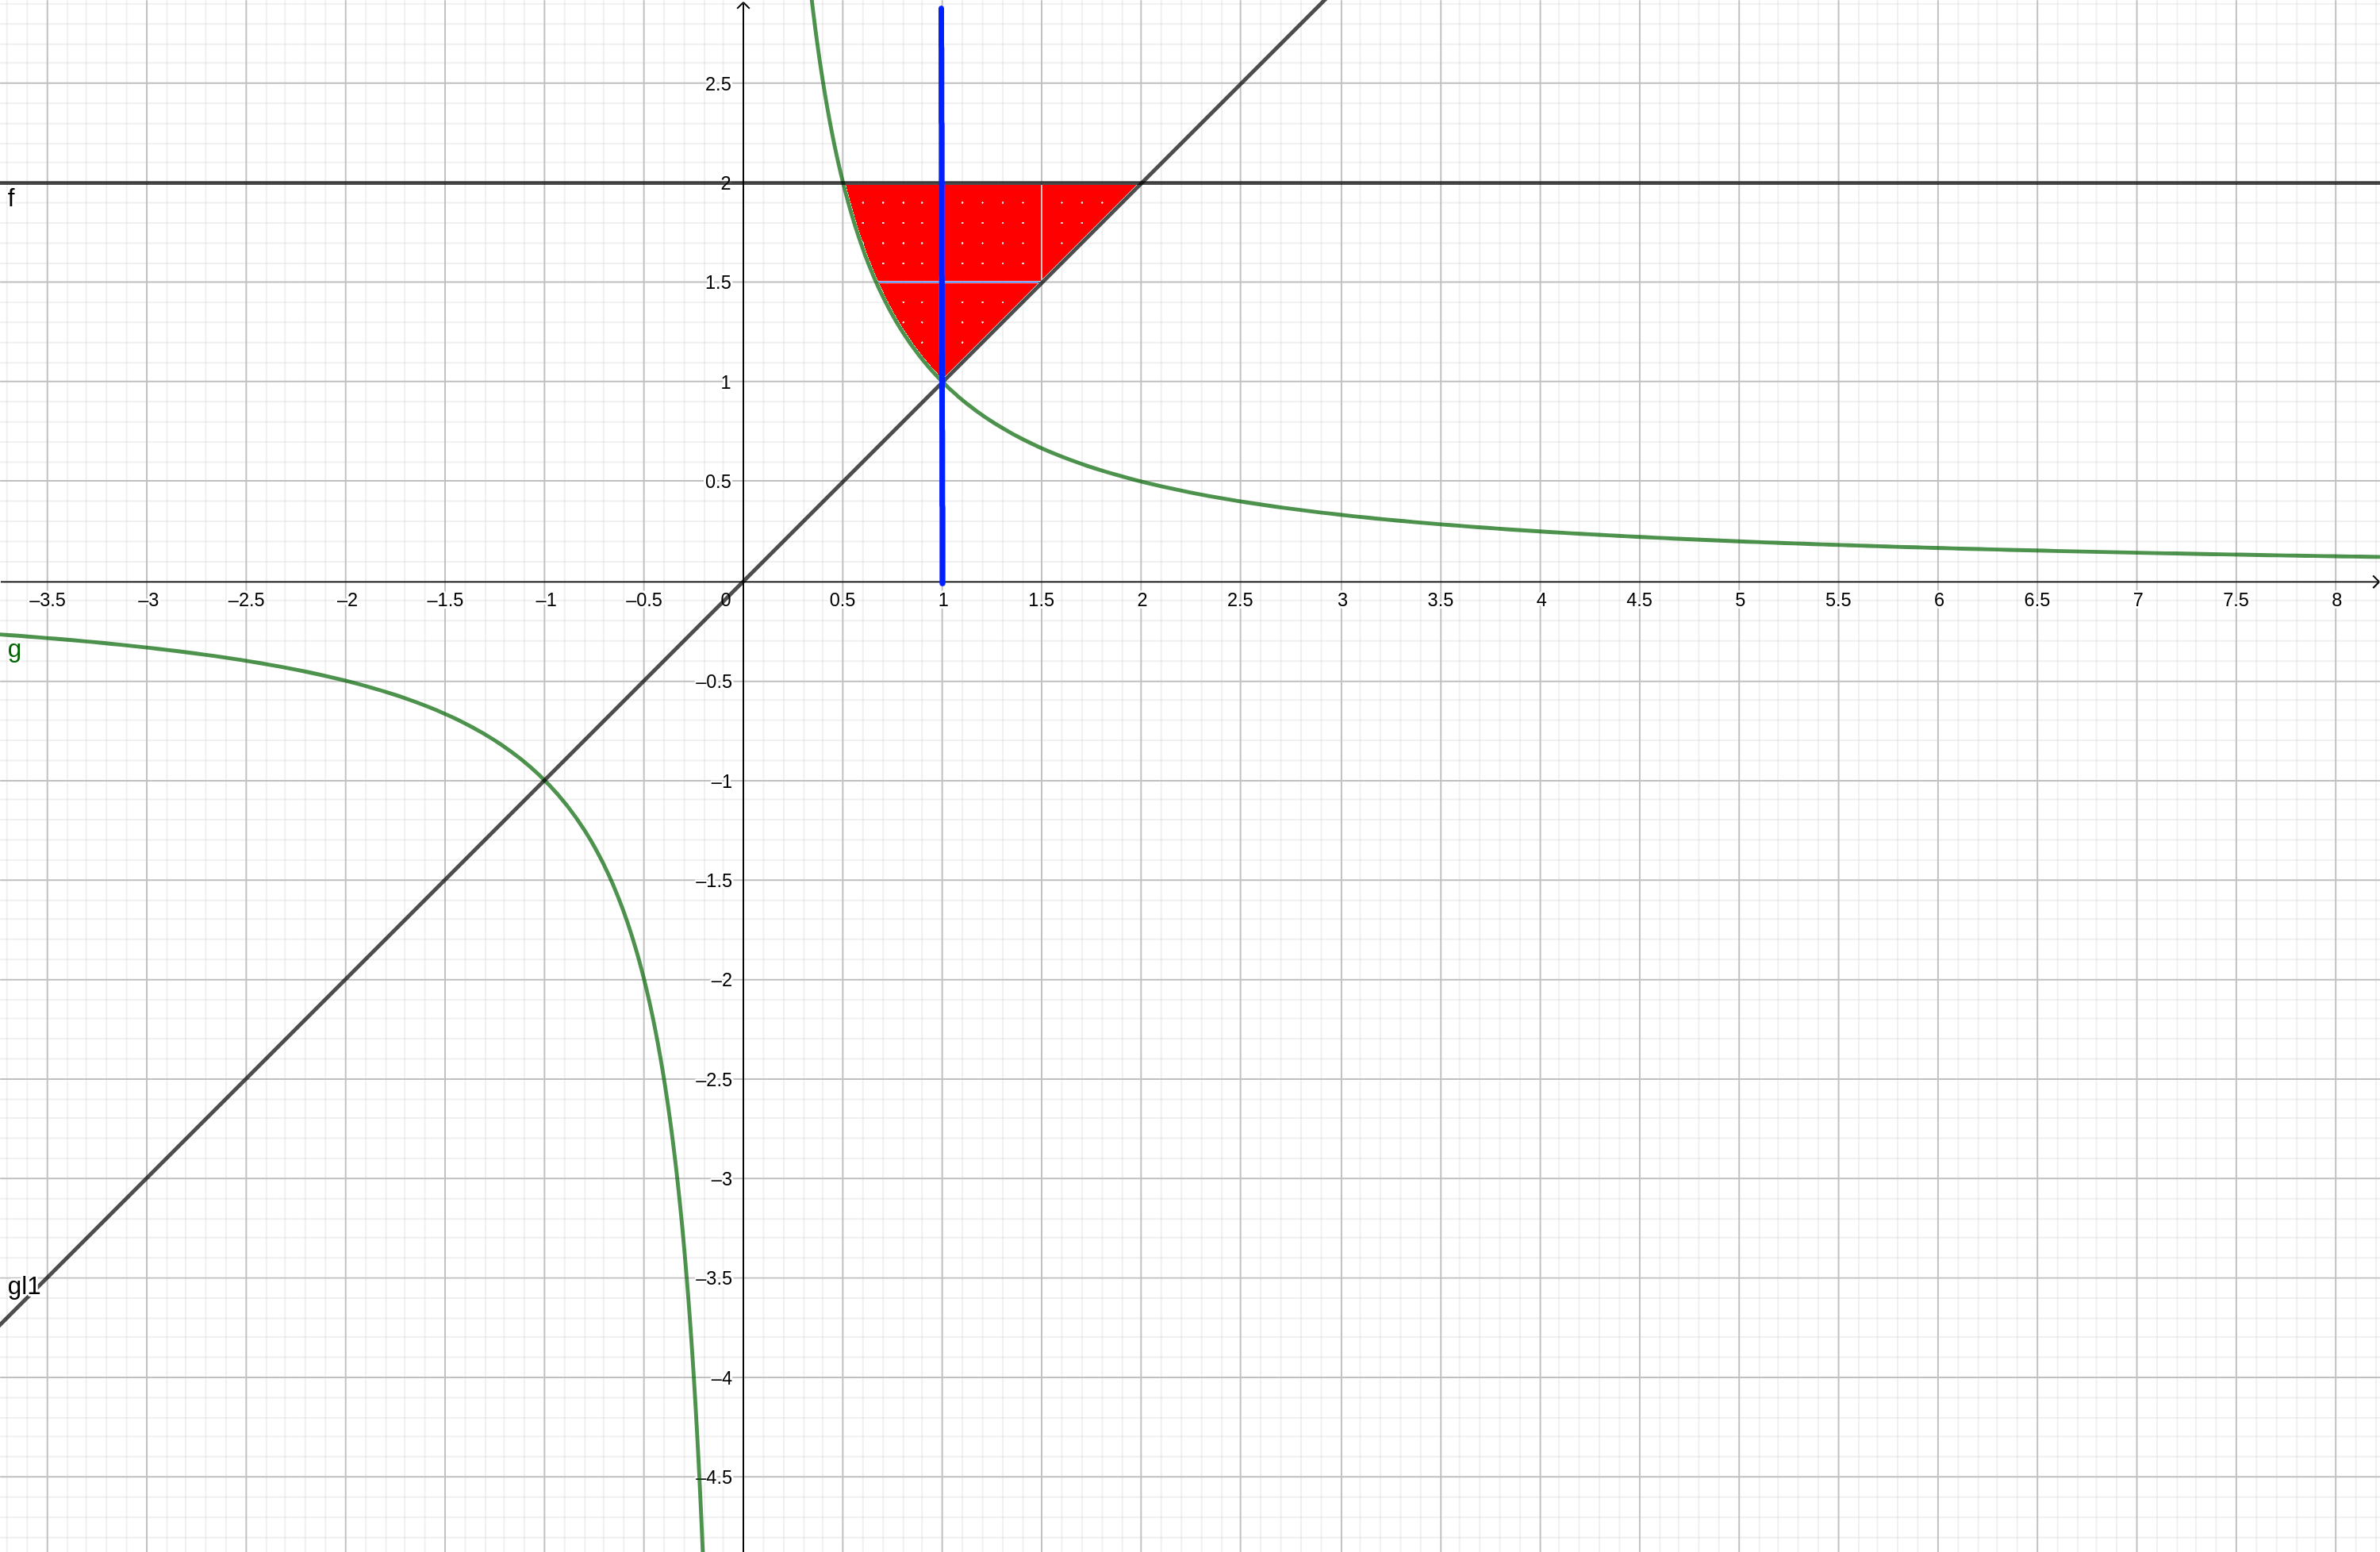
\includegraphics{MengeG.png}
	ii)\\
	$G_1 = \{x\in \mathbb{R}^2| 0.5\leq x_1\leq 1, \frac{1}{x_1} \leq x_2\leq 2\}$\\
	$G_2 = \{x\in \mathbb{R}^2| 1\leq x_1\leq 1.5, x_1 \leq x_2\leq 2\}$\\
	$G_1\cup G_2 = G$.\\
	b)\\
	zuerst: Rechteck auf ellipse, funktion t(x,y) (nach Vorlesung)\\
	Sei $H = \{(x,y)^T\in\mathbb{R}^2: 0\leq x\leq 2\pi, 0\leq y\leq 1\}$ das Rechteck mit projektion auf G durch
	\[t(x,y)= (ya*sin(x),yb*cos(x))\]
	Jacobi-Matrix:\\
	\[\begin{bmatrix}ya*cos(x)& -yb*sin(x)\\ a*\sin(x)&b*\cos(x)\end{bmatrix}\]
	Die Funktionaldeterminante ist also
	\[Jt(x,y) = ya*cos(x)*b*\cos(x)+yb*sin(x)*a*\sin(x)\]
	\[|Jt(x,y)| = yab*\cos^2(x)+yba*\sin^2(x) = yab(\cos^2(x)+\sin^2(x))=yab\]
	Nach transformationssatz:\\
	$$\int _G f(x,y)d(x,y) = \int_M f(x)*|Jt(x,y)|d(x,y)$$
	$$\int_0^{2\pi}\int_0^1 c\sqrt{1-\frac{(ya*sin(x))^2}{a^2}-\frac{(yb*cos(x))^2}{b^2}}yab\ dydx$$
	$$\int_0^{2\pi}\int_0^1 c\sqrt{1-\frac{y^2a^2*sin(x)^2}{a^2}-\frac{y^2b^2*cos^2(x)}{b^2}}yab\ dydx$$
	$$\int_0^{2\pi}\int_0^1 c\sqrt{1-y^2*\sin^2(x)-y^2*\cos^2(x)}yab\ dydx$$
	Vergleiche oben:\\
	$$\int_0^{2\pi}\int_0^1 c\sqrt{1-y^2}yab\ dydx$$
	$$\int_0^{2\pi}abc\int_0^1 \sqrt{1-y^2}y\ dydx$$
	substitution $1-y^2 = u\implies du = -2y\ dy$\\
	$$\int_0^{2\pi}(\frac{abc}{2}\int_{1-0^2}^{1-1^2} \sqrt{u}\ du)dx$$
	$$\frac{abc}{2}\int_0^{2\pi}(-\int^{0}_{1} \sqrt{u}\ du)dx$$
	$$\frac{-abc}{2}\int_0^{2\pi}([\frac{2}{3}u^\frac{3}{2}]^0_1)dx$$
	$$\frac{-abc}{2}\int_0^{2\pi}(0-\frac{2}{3}1^\frac{3}{2})dx$$
	$$\frac{abc}{2}[\frac{2}{3}1^\frac{3}{2}x]^{2\pi}_0$$
	$$\frac{abc}{2}[\frac{2}{3}x]^{2\pi}_0$$
	$$\frac{abc}{2}(\frac{2}{3}(2\pi)-0)$$
	$$\frac{abc}{2}\frac{2}{3}(2\pi)$$
	$$\frac{2abc}{3}\pi$$
	Zusatzaufgabe:\\
	Zuerst umformen von f:\\
	$$f_{X,Y}(x,y) = (1-e^{-\frac{r^2}{2}})^{-1} \frac{1}{2\pi}\exp(-\frac{1}{2}(x^2+y^2))1_\Omega(x,y)$$
	Man kann am argument der exponentialfunktion sehen, dass sich eine Transformation in polarkoordinaten anbietet:\\
	Nach Übung 
	$$\int_H f(k\cos(\theta), k\sin(\theta))k\ d\theta\ dk$$
	Es wurde k statt wie in der Übung r verwendet, da die funktion $f_{X,Y}(x,y)$ schon einen parameter r für den Radius der Scheibe beinhält.\\
	Ereignis A war (nach Musterlösung):\\
	$A=\{\omega\in\Omega|\sqrt{\omega_2^2+\omega_1^2}<1\}$
	mit $\Theta: A\to G,\ \Theta(k,\theta)=(k\cos(\theta), k\sin(\theta))$\\
	die Jacobi-matrix ist:\\
	$J\Theta = \begin{bmatrix}\cos(\theta)&-k\sin(\theta)\\ \sin(\theta) &k\cos(\theta)\end{bmatrix}$\\
	Dies liefert $|J\Theta| = k$ (determinante wie oben berechnet).\\
	Die funktion $\Theta$ muss nicht nur auf A angewandt werden, sondern auf den gesamten Ergebnisraum
	$$\Omega =\{(\omega_1,\omega_2)\in\mathbb{R}^2|\sqrt{\omega_2^2+\omega_1^2}\leq r\}$$
	dies liefert
	$$\Omega' = \{(k,\theta)\in\mathbb{R}^2|0\leq k\leq r,0\leq\theta\leq 2\pi\}$$
	Wobei das Ereignis $A\subset \Omega$ zu\\
	$$A' = \{(k,\theta)\in\mathbb{R}^2|0\leq k< 1,0\leq\theta\leq 2\pi\}$$
	wird.\\
	Wir integrieren also über:
	$$\int_A  f_{X,Y}(x,y) dA = \int_{A'} f_{X,Y}(k\cos(\theta), k\sin(\theta))k\ dA'$$
	$$\int_{A'} (1-e^{-\frac{r^2}{2}})^{-1} \frac{1}{2\pi}\exp(-\frac{1}{2}((k\cos(\theta))^2+(k\sin(\theta))^2))1_{\Omega'}(k\cos(\theta),k\sin(\theta))k\ dA'$$
	Wir machen eine Fallunterscheidung über $1_{\Omega'}(k\cos(\theta),k\sin(\theta))$ null oder eins.\\
	da bekannt ist, dass $r>1$, ist die Indikatorfunktion immer eins, weshalb der fall Indikator =0 nie auftritt.\\
	$$\int_{A'} (1-e^{-\frac{r^2}{2}})^{-1} \frac{1}{2\pi}\exp(-\frac{1}{2}((k\cos(\theta))^2+(k\sin(\theta))^2))k\cdot 1\ dA'$$
	$$\int_{A'} (1-e^{-\frac{r^2}{2}})^{-1} \frac{1}{2\pi}\exp(-\frac{1}{2}(k^2(\cos^2(\theta)+\sin^2(\theta)))k\ dA'$$
	$$\int_{A'} (1-e^{-\frac{r^2}{2}})^{-1} \frac{1}{2\pi}\exp(-\frac{1}{2}(k^2))k\ dA'$$
	$$\int_0^1\int_0^{2\pi} (1-e^{-\frac{r^2}{2}})^{-1} \frac{1}{2\pi}\exp(-\frac{1}{2}(k^2))k\ d\theta\ dk$$
	$$\int_0^1 2\pi (1-e^{-\frac{r^2}{2}})^{-1} \frac{1}{2\pi}\exp(-\frac{1}{2}(k^2))k\ \ dk$$
	$$2\pi (1-e^{-\frac{r^2}{2}})^{-1} \frac{1}{2\pi}\int_0^1 \exp(-\frac{1}{2}(k^2))k\ \ dk$$
	substitution mit $u=\frac{k^2}{2}\implies du = -kdk$\\
	$$2\pi (1-e^{-\frac{r^2}{2}})^{-1} \frac{1}{2\pi}\int_0^{-\frac{1}{2}} -\exp(u)\ du$$
	$$2\pi (1-e^{-\frac{r^2}{2}})^{-1} \frac{1}{2\pi}[ \exp(u)]_{-\frac{1}{2}}^0$$
	$$2\pi (1-e^{-\frac{r^2}{2}})^{-1} \frac{1}{2\pi}[ 1-\exp(-\frac{1}{2})] =P(A)$$
	Für B kann auch eine projektion auf polarkoordinaten angewandt werden.\\
	Die Form von $\Omega'$ ändert sich damit nicht.\\
	B in polarkoordinaten:\\
	$$B' = \{(k,\theta)\in\mathbb{R}^2| 0\leq k\leq r, 0\leq \theta\leq \frac{\pi}{2} \}$$
	Das $\frac{\pi}{2}$ entsteht, weil B das Ereignis der Pfeile im ersten Quadranten ist (was von $0$ bis $\frac{\pi}{2}$ reicht)\\
	$$\int_B  f_{X,Y}(x,y) dB = \int_{B'} f_{X,Y}(k\cos(\theta), k\sin(\theta))k\ dB'$$
	$$\int_0^r\int_0^\frac{\pi}{2} (1-e^{-\frac{r^2}{2}})^{-1} \frac{1}{2\pi}\exp(-\frac{1}{2}((k\cos(\theta))^2+(k\sin(\theta))^2))1_{\Omega'}(k\cos(\theta),k\sin(\theta))k\ d\theta dr $$
	Auch hier muss technisch gesehen zwischen $1_{\Omega'}(k\cos(\theta),k\sin(\theta)) =0$ und $1_{\Omega'}(k\cos(\theta),k\sin(\theta))=1$ unterschieden werden. Da aber für den ersten Fall das integral sowieso null ist kann  man diesen Teil des integrals vernachlässigen: $\int 0 dx = 0$\\
	$$\int_0^r\int_0^\frac{\pi}{2} (1-e^{-\frac{r^2}{2}})^{-1} \frac{1}{2\pi}\exp(-\frac{1}{2}k^2)k\ d\theta dr $$
	$$\int_0^r\frac{\pi}{2} (1-e^{-\frac{r^2}{2}})^{-1} \frac{1}{2\pi}\exp(-\frac{1}{2}k^2)k\ dr $$
	$$(1-e^{-\frac{r^2}{2}})^{-1} \frac{1}{2\pi}\frac{\pi}{2}\int_0^r \exp(-\frac{1}{2}k^2)k\ dr $$
	substitution mit $u=\frac{k^2}{2}\implies du = -kdk$\\
	$$(1-e^{-\frac{r^2}{2}})^{-1} \frac{1}{4}\int_0^{-\frac{r^2}{2}} -\exp(u)\ du$$
	$$(1-e^{-\frac{r^2}{2}})^{-1} \frac{1}{4}[ \exp(u)]^0_{-\frac{r^2}{2}}$$
	$$(1-e^{-\frac{r^2}{2}})^{-1} \frac{1}{4}[1- \exp({-\frac{r^2}{2}})] = \frac{1}{4}=P(B)$$
\end{document}